\documentclass[11pt]{article}

\usepackage[T1]{fontenc}
\usepackage[utf8]{inputenc}
\usepackage{lmodern}
\usepackage{microtype}
\usepackage[a4paper,margin=29mm]{geometry}
\usepackage{amsmath,amssymb,amsthm,mathtools}
\usepackage{booktabs,array,longtable}
\usepackage{enumitem}
\usepackage{tikz}
\usepackage{pgfplots}
\pgfplotsset{compat=1.18}
\usepackage{xcolor}
\usepackage{hyperref}
\usepackage[nameinlink,capitalise,noabbrev]{cleveref}
\usepackage{listings}
\usepackage{url}
% Author information for arXiv submission.
\newcommand{\PaperAuthor}{Vladislav Kuznetsov}
\newcommand{\PaperAffiliation}{Moscow Institute of Physics and Technology (MIPT), Dolgoprudny, Russia}
\newcommand{\PaperEmail}{vladkuznecov266@gmail.com}


\hypersetup{
  colorlinks=true,
  linkcolor=blue!55!black,
  citecolor=blue!55!black,
  urlcolor=blue!55!black,
  pdftitle={The Exact Worst-Case Color-Neutral Distance for the First Block Phase of the Megaminx},
  pdfauthor={\PaperAuthor}
}
\setlist{nosep}
\lstset{basicstyle=\ttfamily\small,breaklines=true,columns=fullflexible}

\newtheorem{theorem}{Theorem}
\newtheorem{lemma}[theorem]{Lemma}
\newtheorem{corollary}[theorem]{Corollary}
\newtheorem{proposition}[theorem]{Proposition}
\theoremstyle{definition}
\newtheorem{definition}[theorem]{Definition}
\newtheorem{remark}[theorem]{Remark}

\newcommand{\FTM}{\mathrm{FTM}}
\newcommand{\DCN}{D_{\mathrm{CN}}}
\newcommand{\dCN}{d_{\mathrm{CN}}}

\title{The Exact Worst-Case Color-Neutral Distance for the First Block Phase of the Megaminx}
\author{\PaperAuthor\\\small \PaperAffiliation\\\small \texttt{\PaperEmail}}
\date{July 2026}

\begin{document}
\maketitle

\begin{abstract}
We study the first phase of a recently developed multi-phase Megaminx solver in the face-turn metric.  For a fixed target corner, this phase solves that corner together with its three incident edge pieces.  Its phase-coordinate graph has $11{,}692{,}800$ vertices; the maximum distance from the solved coordinate is $10$, attained by exactly $159$ vertices.  We allow the target corner to be selected adaptively among all $20$ corners of the puzzle.  An exhaustive compatibility computation shows that no reachable Megaminx state places all $20$ target blocks at distance $10$: after discarding all corner constraints, only five globally compatible edge configurations remain, and every one has odd edge-permutation parity.  Conversely, we give a reachable full state whose distance is exactly $9$ for every target corner.  Hence the worst-case color-neutral distance of this phase is exactly
\[
\DCN=9.
\]
Conditional on the previously reported $114$-move face-turn bound, this one-move reduction gives the corresponding conditional bound of $113$ moves.  Source code, certificates, two independently implemented exhaustive CSP enumerators, an independent Schreier--Sims reachability verifier, and a one-command reproduction script accompany the paper.
\end{abstract}

\section{Introduction}

The Megaminx is the dodecahedral analogue of the Rubik's Cube.  It has $20$ movable corner pieces and $30$ movable edge pieces, and its full state graph is far too large for direct breadth-first search.  As for the Rubik's Cube, practical upper bounds are therefore obtained by a chain of subgroup or quotient-space reductions, with a shortest-path table for each phase.  Adding the worst-case length of each phase gives a rigorous upper bound whenever every table and the terminal step have been exhaustively certified.

Botz developed and published a computational Megaminx solver based on this approach~\cite{botz-software,botz-thread}.  His shortened phase chain gives
\[
10+15+14+8+13+13+17+26=116.
\]
The last term comes from Whitmore's reported two-generator computation, which Botz did not independently reproduce in the thesis, so $116$ was a conditional, publicly reported face-turn bound~\cite{botz-software,botz-116}.  A forum exchange briefly suggested $117$ because one displayed table appeared to reach depth $14$; Botz later clarified that the duplicated rows were a transcription error and that the table ended at $13$, consistently with the thesis~\cite{botz-116-correction}.  Rokicki later reported $24$-move solutions for all $16$ distance-$26$ two-generator positions after admitting a third face.  Since distance-$25$ positions remained, this reduced the last-phase guarantee from $26$ to $25$ and the total from $116$ to $115$~\cite{rokicki-115}.  He then reported that all $7{,}595$ distance-$25$ positions, reduced to $1{,}199$ representatives by symmetry and inversion, are solvable in at most $24$ moves; this reduced the last-phase guarantee to $24$ and the total to $114$~\cite{rokicki-114}.  Botz later identified $114$ as the improved value~\cite{botz-114}.  These announcements are currently the public record of that bound rather than a refereed proof.

This paper isolates and certifies one further improvement.  The original first phase chooses a fixed corner and solves the corner piece together with its three incident edges.  A human solver would naturally choose the most favorable starting corner.  We formalize that freedom and prove that it lowers the worst-case first-phase cost from $10$ to exactly $9$.

The contribution is deliberately narrow:
\begin{enumerate}
  \item we reproduce the complete fixed-target distance distribution;
  \item we prove an exhaustive upper bound of $9$ for the adaptive, or color-neutral, phase;
  \item we provide a reachable witness establishing the matching lower bound;
  \item we state the resulting conditional one-move improvement to the announced global bound.
\end{enumerate}
The computational proof follows a standard pattern: an expensive search produces compact certificates that are checked by small, independent programs~\cite{rokicki2013,kunkle2007}.

\section{Megaminx states and metric}

A Megaminx face turn cyclically permutes the five corners and five edges incident with a face.  We use the \emph{face-turn metric}: any nonzero power of a face turn, namely $72^\circ$, $144^\circ$, $216^\circ$, or $288^\circ$, has length one.  Thus each of the $12$ faces supplies four moves.

We index corner pieces and corner positions by $\{0,\ldots,19\}$ and edge pieces and edge positions by $\{0,\ldots,29\}$.  Corner orientations lie in $\mathbb Z/3\mathbb Z$ and edge orientations in $\mathbb Z/2\mathbb Z$.  We use the standard reachability characterization of the Megaminx move group: a cubie assignment is reachable exactly when both the corner and edge permutations are even and the total corner and edge orientations are respectively zero modulo $3$ and $2$~\cite[Theorems 3.8 and 3.12]{xu2018}.  Equivalently, the move group has the structure
\[
\left((\mathbb Z/3\mathbb Z)^{19}\times(\mathbb Z/2\mathbb Z)^{29}\right)
\rtimes\left(A_{20}\times A_{30}\right).
\]
Only the necessity of even edge parity is used for the upper bound; the full characterization is used to certify the lower-bound witness.

\section{The fixed-target first phase}

Fix a target corner $v$ and let $e_1,e_2,e_3$ be its three incident target edge pieces.  A phase coordinate records
\[
(c,o_c,p_1,p_2,p_3,o_1,o_2,o_3),
\]
where $c$ and $o_c$ are the current position and orientation of the target corner and $p_i,o_i$ are the current position and orientation of target edge $e_i$.  The three edge positions are distinct.  Consequently the coordinate space has
\begin{align*}
|X|&=20\cdot 3\cdot(30\cdot29\cdot28)\cdot2^3\\
&=11{,}692{,}800
\end{align*}
vertices.  This agrees with the coordinate allocation and ranking formula in the public first-phase implementation~\cite{botz-12gen}.

The phase-coordinate graph $\Gamma_v$ on $X$ is generated by all $48$ face-turn-metric moves.  A complete breadth-first search from the solved target coordinate gives the distribution in \cref{tab:distribution}.  Our implementation visits every coordinate exactly once.  Thus the solved coordinate has eccentricity $10$.  All $20$ target choices have the same distance distribution, and full regenerations from source produced byte-identical binary certificate files for every target.

\begin{table}[ht]
\centering
\caption{Distance distribution for a fixed first-block target.}
\label{tab:distribution}
\begin{tabular}{@{}rr@{}}
\toprule
Distance & States\\
\midrule
0 & 1\\
1 & 12\\
2 & 168\\
3 & 2,214\\
4 & 26,466\\
5 & 256,292\\
6 & 1,668,044\\
7 & 5,125,524\\
8 & 4,249,463\\
9 & 364,457\\
10 & 159\\
\midrule
Total & 11,692,800\\
\bottomrule
\end{tabular}
\end{table}

\begin{remark}[Cayley versus Schreier graph]
The full Megaminx state graph is a Cayley graph of the move group, but $\Gamma_v$ is a Schreier graph for the action of that group on the phase coordinates, equivalently on cosets of the stabilizer of the tracked block.  This stabilizer is not normal, so the coordinates do not themselves form a quotient group, and the Schreier graph need not be vertex-transitive.  Here the distinction is visible: an exhaustive orbit-reduced computation gives
\[
\operatorname{diam}(\Gamma_v)=11,
\]
even though the solved coordinate has eccentricity $10$.  The computation normalizes orientations and tracked-edge labels, reduces the resulting $81{,}200$ positional roots by the $120$ spatial symmetries to $708$ orbit representatives, and runs a complete BFS from each representative.  Of these representatives, $637$ have eccentricity $10$ and $71$ have eccentricity $11$.  These counts refer to orbit representatives, not to vertices.  Source and a machine-readable result are included in the artifact.  This ordinary graph diameter is not used in the color-neutral argument below.
\end{remark}

\begin{figure}[ht]
\centering
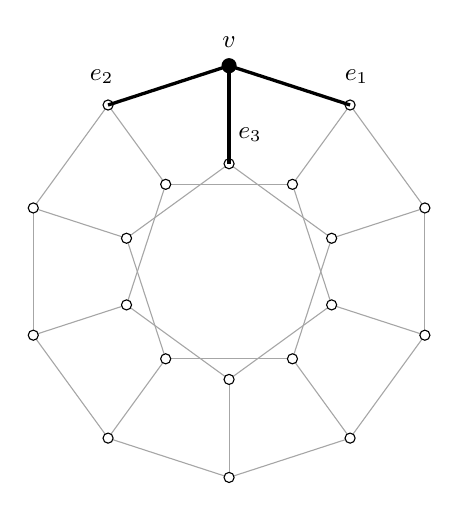
\begin{tikzpicture}[scale=0.83, every node/.style={font=\small}]
  % Dodecahedral graph as generalized Petersen graph G(10,2).
  \foreach \i in {0,...,9} {
    \coordinate (o\i) at ({90-36*\i}:3.15);
    \coordinate (i\i) at ({90-36*\i}:1.65);
  }
  \foreach \i in {0,...,9} {
    \pgfmathtruncatemacro{\j}{mod(\i+1,10)}
    \draw[gray!70] (o\i)--(o\j);
    \draw[gray!70] (o\i)--(i\i);
    \pgfmathtruncatemacro{\k}{mod(\i+2,10)}
    \draw[gray!70] (i\i)--(i\k);
  }
  \foreach \i in {0,...,9} {
    \fill[white] (o\i) circle (2.2pt);
    \draw (o\i) circle (2.2pt);
    \fill[white] (i\i) circle (2.2pt);
    \draw (i\i) circle (2.2pt);
  }
  \draw[very thick] (o0)--(o1);
  \draw[very thick] (o0)--(o9);
  \draw[very thick] (o0)--(i0);
  \fill (o0) circle (3.3pt) node[above=3pt] {$v$};
  \node at (1.95,2.98) {$e_1$};
  \node at (-1.95,2.98) {$e_2$};
  \node at (0.32,2.1) {$e_3$};
\end{tikzpicture}
\caption{The dodecahedral corner-edge incidence graph.  Each of its $20$ vertices defines a possible first-block target: one corner $v$ and its three incident edges.}
\label{fig:dodecahedral-graph}
\end{figure}

\section{Color-neutral distance}

Let $V$ be the set of $20$ target corners.  For a reachable full state $g$, let $q_v(g)\in X_v$ be its local phase coordinate for target $v$, and let $d_v(g)$ be the graph distance of that coordinate from the solved target coordinate.  The $20$ graphs $X_v$ are mutually isomorphic under physical rotations of the dodecahedron.

\begin{definition}
The color-neutral first-phase distance and its worst-case value are
\[
\dCN(g)=\min_{v\in V}d_v(g),
\qquad
\DCN=\max_{g}\dCN(g),
\]
where the maximum ranges over reachable full Megaminx states.
\end{definition}

Since the solved coordinate has eccentricity $10$ for every fixed target, trivially $\DCN\le10$.  The issue is whether a full state can project to a depth-$10$ coordinate for all $20$ targets simultaneously.

\section{Upper bound: no simultaneous depth-$10$ state}

For each target $v$, let $A_v\subset X_v$ denote its $159$ depth-$10$ coordinates.  Suppose for contradiction that a reachable full state $g$ satisfies $d_v(g)=10$ for every $v$.  Then
\[
q_v(g)\in A_v\quad\text{for all }v\in V.
\]
We now discard information and solve a relaxed compatibility problem.

\subsection{Edge-signature relaxation}

Project each element of $A_v$ onto the positions and orientations of the three target edges incident with $v$, forgetting the target corner entirely.  Although $|A_v|=159$, this projection has only $80$ distinct edge signatures for every target.

Every physical target edge belongs to exactly two target blocks, one at each endpoint of the edge in \cref{fig:dodecahedral-graph}.  A globally consistent selection of one signature per block must satisfy:
\begin{enumerate}
  \item the two endpoint blocks assign the same position and orientation to their shared target edge;
  \item the $30$ target edge pieces occupy $30$ distinct positions.
\end{enumerate}
We impose no corner constraints and no reachability constraints.  Thus every hypothetical Megaminx state whose $20$ projections all have depth $10$ gives a solution of this relaxed constraint system, but the converse need not hold.

\subsection{Exhaustive enumeration}

Two independent implementations enumerate the relaxation.  The Python implementation uses arc consistency, singleton propagation for the global all-different constraint, and minimum-remaining-values branching.  The C++ implementation performs a separate block-domain backtracking search with dynamic minimum-domain selection and explicit global edge-position ownership.  They visit $145$ and $1{,}015$ search nodes respectively and return exactly the same five configurations.

For all five, the edge permutation has cycle type
\[
2^3 3^8,
\]
that is, three disjoint transpositions and eight disjoint $3$-cycles.  In particular every configuration is odd.  The five permutations, in piece-to-position notation, are included in \cref{app:five-configurations} and as machine-readable certificates.

\begin{lemma}
Every reachable Megaminx state has an even edge permutation.
\end{lemma}
\begin{proof}
A face turn acts on edge positions as a $5$-cycle.  A $5$-cycle has sign $(-1)^{5-1}=+1$, so every generator is even.  Products of the generators are therefore even.
\end{proof}

\begin{proposition}\label{prop:upper}
$\DCN\le9$.
\end{proposition}
\begin{proof}
If a reachable state had distance $10$ for all $20$ targets, its edge assignment would occur among the solutions of the relaxation.  Exhaustive enumeration leaves exactly five possibilities, and all five have odd edge permutation.  The lemma excludes every one of them.  Hence every reachable state has at least one target at distance at most $9$.
\end{proof}

The logical role of the computation is limited and checkable: it enumerates a finite CSP with $20$ variables and $80$ values per variable, and outputs all five solutions.  The parity exclusion itself is elementary.

\section{Lower bound: a state with twenty distances equal to nine}

To show that the upper bound is sharp, we provide the full cubie state $g_\star$ listed in \cref{app:witness}.  Its corner and edge permutations are both even, its corner-orientation sum is $0\pmod 3$, and its edge-orientation sum is $0\pmod 2$.  These invariants imply reachability by the characterization recalled in \cref{sec:reachability-note}.  The artifact additionally supplies an independent Schreier--Sims check: it represents the twelve face generators on the $120$ oriented cubie-position states, computes a group of order
\[
\frac{20!}{2}3^{19}\,\frac{30!}{2}2^{29},
\]
verifies that this equals the full invariant-compatible state count, and directly confirms that the permutation representing $g_\star$ belongs to the generated group.

For each target $v$, two independently written witness verifiers form $q_v(g_\star)$ and check two sorted certificate sets generated by the complete BFS:
\begin{enumerate}
  \item $q_v(g_\star)$ occurs in the union of the depth-$9$ and depth-$10$ layers;
  \item $q_v(g_\star)$ does not occur in the depth-$10$ layer.
\end{enumerate}
Therefore $d_v(g_\star)=9$ for every one of the $20$ targets.  The resulting distance vector is
\[
(9,9,9,9,9,9,9,9,9,9,9,9,9,9,9,9,9,9,9,9).
\]

\begin{proposition}\label{prop:lower}
$\DCN\ge9$.
\end{proposition}
\begin{proof}
The reachable witness $g_\star$ satisfies $\dCN(g_\star)=9$.
\end{proof}

Combining \cref{prop:upper,prop:lower} gives the main result.

\begin{theorem}\label{thm:main}
The exact worst-case color-neutral distance of the first corner-block phase is
\[
\boxed{\DCN=9}.
\]
\end{theorem}

\section{Consequence for the global upper bound}

The adaptive target does not add a physical move.  It selects a reference frame.  Let
\[
G=G_0\supset G_1\supset\cdots\supset G_k=\{1\}
\]
be a canonical phase chain whose first target is one fixed corner block.  If a rotation $\rho$ maps the canonical target to another target $v$, then
\[
G_i^{(v)}=\rho G_i\rho^{-1}
\]
is a conjugate phase chain.  Physical rotations permute the $12$ face generators and preserve face-turn length, so every phase worst-case bound and every terminal worst-case guarantee is unchanged under this conjugation.

Thus, for each input state, one may select a target $v$ attaining $\dCN(g)$, use at most nine moves for the first phase, and continue through the correspondingly relabelled chain with exactly the same bounds as before.

\begin{corollary}[Conditional on the reported $114$-move computation]\label{cor:113}
If the external computations underlying the reported $114$-move face-turn upper bound for the eight-phase construction are valid, then the same construction with the color-neutral first phase gives the conditional bound
\[
\operatorname{diam}_{\FTM}(\text{Megaminx})\le 113.
\]
\end{corollary}
\begin{proof}
In the announced construction, the fixed first phase contributes $10$ moves.  By \cref{thm:main} it can be replaced by its color-neutral version, which contributes at most $9$, while rotational conjugacy preserves all later phase guarantees.  Hence $114-1=113$.
\end{proof}

\begin{remark}
The accompanying artifact independently verifies the new first-phase result but does not re-run the much larger computations underlying the reported $114$-move bound.  Accordingly, the number $113$ is a conditional consequence of that external computation, whereas \cref{thm:main} is independently certified here.
\end{remark}

\section{Reproducibility}

The artifact contains:
\begin{itemize}
  \item an independent C++ implementation of the phase coordinate and all $12$ face moves;
  \item a complete BFS generator for all $20$ target blocks;
  \item an orbit-reduced exhaustive checker for the ordinary coordinate-graph diameter;
  \item the $20$ depth-$10$ sets and the $20$ top-two-layer sets;
  \item independent Python and C++ exhaustive CSP solvers;
  \item the full-state lower-bound witness, two layer-membership verifiers, and an independent Schreier--Sims group-membership verifier;
  \item byte-level checksums and one-command scripts for quick verification and full regeneration.
\end{itemize}

On the audit machine, a single target table was generated in approximately $5$--$6$ seconds using about $65$ MiB of memory.  The four-worker full regeneration remained below $300$ MiB.  These timings are informative only; the proof depends on the deterministic output and certificate checks, not on performance.

The quick check is
\begin{lstlisting}
./scripts/quick_verify.sh
\end{lstlisting}
and the full regeneration is
\begin{lstlisting}
./scripts/reproduce.sh
\end{lstlisting}
The latter rebuilds all $20$ tables, requires the regenerated files to be byte-identical to the distributed certificates, and rechecks the ordinary coordinate-graph diameter.

\section{Acknowledgements}

The author used OpenAI's ChatGPT to assist with software development, manuscript editing, and the organization of computational verification.  The author takes responsibility for all mathematical claims, computations, source references, and conclusions.

\section{Conclusion}

The solved coordinate of the fixed first-block phase has eccentricity $10$, but its depth-$10$ set is too sparse and too incompatible across the $20$ possible targets to occur simultaneously in a legal full state.  A relaxed edge-only CSP reduces all putative counterexamples to five configurations, and an edge-parity invariant excludes all five.  A legal state at distance $9$ from every target proves sharpness.  Therefore the exact worst-case color-neutral first-phase distance is $9$.  Conditional on the previously reported $114$-move computation, this yields the corresponding one-move reduction to $113$.

\appendix

\section{Reachability note}\label{sec:reachability-note}

For completeness, the lower-bound certificate uses the following standard characterization~\cite{xu2018}.  If corners and edges are represented independently, a cubie state is reachable precisely when
\begin{align*}
\operatorname{sgn}(\pi_C)&=+1,& \sum_{i=0}^{19}o_C(i)&=0\pmod 3,\\
\operatorname{sgn}(\pi_E)&=+1,& \sum_{i=0}^{29}o_E(i)&=0\pmod 2.
\end{align*}
Necessity follows immediately from the action of one face turn.  Sufficiency follows by generating arbitrary corner and edge $3$-cycles and arbitrary paired corner twists and paired edge flips; these generate $A_{20}$, $A_{30}$, $(\mathbb Z/3\mathbb Z)^{19}$, and $(\mathbb Z/2\mathbb Z)^{29}$ respectively.  The distributed layer-membership verifiers check all four conditions for $g_\star$.  Independently, the Schreier--Sims verifier constructs the group generated by the twelve face turns on oriented cubie-position states, checks that its order equals the invariant-compatible state count above, and tests $g_\star$ for group membership directly.

\section{Lower-bound witness}\label{app:witness}

The arrays below map each piece index to its occupied position.  Orientations are indexed by piece in the same order.

\noindent\textbf{Corner piece to position.}\par
\begin{lstlisting}
18 19 11 13 8 1 2 0 5 7 12 3 6 10 17 4 16 9 14 15
\end{lstlisting}
\noindent\textbf{Corner orientation.}\par
\begin{lstlisting}
0 1 0 1 0 1 0 0 0 2 2 2 1 1 2 0 0 2 0 0
\end{lstlisting}
\noindent\textbf{Edge piece to position.}\par
\begin{lstlisting}
3 18 10 6 29 13 22 25 17 23 11 28 14 16 24
9 27 19 20 1 12 8 0 21 5 4 7 15 2 26
\end{lstlisting}
\noindent\textbf{Edge orientation.}\par
\begin{lstlisting}
1 1 1 0 1 0 0 0 0 1 0 1 0 0 1
0 0 1 1 0 1 1 1 1 1 0 0 0 1 1
\end{lstlisting}

\section{The five relaxed edge configurations}\label{app:five-configurations}

Each row maps edge pieces $0,1,\ldots,29$ to positions.  Every row has cycle type $2^3 3^8$ and odd parity.

\begin{enumerate}[leftmargin=2em]
\item {\ttfamily\footnotesize\raggedright 13 26 16 27 25 19 23 20 11 24 18 21 4 29 6 3 28 7 10 22 17 8 5 14 9 12 1 15 2 0\par}
\item {\ttfamily\footnotesize\raggedright 18 29 27 11 28 22 14 21 16 20 2 26 9 15 23 13 24 1 25 5 12 7 19 6 8 0 3 10 4 17\par}
\item {\ttfamily\footnotesize\raggedright 25 28 10 29 19 13 22 17 21 23 27 8 16 24 1 9 12 20 0 26 7 11 6 15 5 18 4 2 14 3\par}
\item {\ttfamily\footnotesize\raggedright 27 17 28 26 12 24 21 10 20 15 22 3 25 5 19 23 2 29 6 14 8 18 7 9 13 4 11 0 16 1\par}
\item {\ttfamily\footnotesize\raggedright 29 14 25 15 26 23 18 22 24 12 7 17 20 0 28 27 8 11 21 4 9 6 10 5 16 2 19 3 1 13\par}
\end{enumerate}

\begin{thebibliography}{99}

\bibitem{botz-software}
A. Botz,
\newblock \emph{A Megaminx Solver},
\newblock software dataset, TUdatalib, 2026.
\newblock \url{https://tudatalib.ulb.tu-darmstadt.de/handle/tudatalib/5015}.

\bibitem{botz-thread}
A. Botz,
\newblock ``Development of a Megaminx solver,''
\newblock SpeedSolving Puzzles Community, 2024--2026.
\newblock \url{https://www.speedsolving.com/threads/development-of-a-megaminx-solver.93202/}.

\bibitem{botz-116}
A. Botz,
\newblock forum post reporting the merged-phase $116$-move bound,
\newblock February 27, 2025.
\newblock \url{https://www.speedsolving.com/threads/development-of-a-megaminx-solver.93202/post-1645809}.

\bibitem{botz-116-correction}
A. Botz,
\newblock forum post correcting the displayed depth-$14$ table to depth $13$,
\newblock September 22, 2025.
\newblock \url{https://www.speedsolving.com/threads/development-of-a-megaminx-solver.93202/post-1670603}.

\bibitem{rokicki-115}
T. Rokicki,
\newblock forum post giving $24$-move solutions for all $16$ distance-$26$ two-generator positions,
\newblock November 6, 2025.
\newblock \url{https://www.speedsolving.com/threads/development-of-a-megaminx-solver.93202/post-1675762}.

\bibitem{rokicki-114}
T. Rokicki,
\newblock forum post reporting solutions of the $7{,}595$ distance-$25$ two-generator positions in at most $24$ moves,
\newblock November 8, 2025.
\newblock \url{https://www.speedsolving.com/threads/development-of-a-megaminx-solver.93202/post-1675972}.

\bibitem{botz-114}
A. Botz,
\newblock forum post identifying $114$ as the improved upper bound,
\newblock March 2026.
\newblock \url{https://www.speedsolving.com/threads/development-of-a-megaminx-solver.93202/post-1690628}.

\bibitem{botz-12gen}
A. Botz,
\newblock \texttt{12Gen.go}, public source-code commit for the first-phase coordinate,
\newblock 2025.
\newblock \url{https://git.rwth-aachen.de/alexander.botz/megaminx-solver-v2.0/-/commit/8ff4cafbf24632cbada2a5f63e447c9982ddf0e4}.

\bibitem{xu2018}
G. J. Xu,
\newblock ``Solving Megaminx Puzzle with Group Theory,''
\newblock preprint submitted to the Yau High School Mathematics Competition, 2018.
\newblock \url{https://oss.linstitute.net/wechatimg/2018/07/qiuchengtong2018mathgold.pdf}.

\bibitem{rokicki2013}
T. Rokicki, H. Kociemba, M. Davidson, and J. Dethridge,
\newblock ``The diameter of the Rubik's Cube group is twenty,''
\newblock \emph{SIAM Journal on Discrete Mathematics}, 27(2):1082--1105, 2013.
\newblock \url{https://doi.org/10.1137/120867366}.

\bibitem{kunkle2007}
D. Kunkle and G. Cooperman,
\newblock ``Twenty-six moves suffice for Rubik's Cube,''
\newblock in \emph{Proceedings of ISSAC 2007}, pages 235--242, ACM, 2007.
\newblock \url{https://doi.org/10.1145/1277548.1277581}.

\end{thebibliography}

\end{document}
